\section{Algoritmos Genéticos}
\label{sec:2.3}

Este tópico apresenta os fundamentos dos Algoritmos Genéticos a partir de duas perspectivas complementares. Inicialmente, são abordados os conceitos biológicos que inspiram essa classe de algoritmos, como população, indivíduo, variabilidade genética, herança, seleção natural, recombinação, mutação e evolução ao longo de gerações. Em seguida, discute-se como esses conceitos são abstraídos e adaptados para o campo computacional, dando origem a mecanismos de busca e otimização aplicáveis a problemas complexos.

\subsection{Fundamentação Biológica}
\label{subsec:fundamentacao-biologica}

A evolução biológica ocorre em populações de indivíduos que apresentam diferenças hereditárias entre si. De acordo com \citeonline{futuyma2023}, essas diferenças constituem a base da variação evolutiva, pois podem influenciar a sobrevivência e a reprodução dos organismos em determinado ambiente. Ao longo das gerações, características associadas a maior sucesso reprodutivo tendem a se tornar mais frequentes na população.

Segundo o renomado autor \citeonline{darwin1859}, a teoria da evolução por seleção natural constitui a base para a compreensão desse processo, ao demonstrar que indivíduos com características mais favoráveis às condições ambientais tendem a deixar mais descendentes. Posteriormente, os avanços da genética permitiram explicar como características são transmitidas, recombinadas e modificadas entre gerações. Sob o olhar de \citeonline{pierce2024}, conceitos como herança genética, genótipo, fenótipo, recombinação e mutação são fundamentais para compreender a transmissão e a variação das características biológicas. Assim, população, indivíduo, variabilidade genética, herança, genótipo, fenótipo, recombinação, mutação e seleção natural formam a base conceitual necessária para compreender os princípios biológicos que inspiram os Algoritmos Genéticos.

\subsubsection{População, Indivíduo e Ambiente}
\label{subsubsec:populacao-individuo-ambiente}

Na biologia, uma população é formada por indivíduos de uma mesma espécie que compartilham determinado ambiente e participam de processos reprodutivos. Como afrima \citeonline{futuyma2023}, a evolução não ocorre em indivíduos isolados, mas em populações ao longo de gerações, por meio da alteração na frequência de características hereditárias.

Cada indivíduo possui características próprias, algumas herdadas geneticamente, que podem influenciar sua adaptação ao ambiente. Com isso \citeonline{urry2021} diz que, o ambiente exerce influência direta sobre a sobrevivência e a reprodução dos organismos, atuando como fonte de pressão seletiva. Essa adaptação não deve ser entendida como superioridade absoluta, mas como adequação relativa a condições específicas.

\subsubsection{Variabilidade Genética}
\label{subsubsec:variabilidade-genetica}

A variabilidade genética corresponde às diferenças hereditárias existentes entre os indivíduos de uma população. Segundo \citeonline{futuyma2023}, essa variabilidade é essencial para a evolução, pois fornece o conjunto de diferenças sobre o qual a seleção natural pode atuar.

Sem variabilidade, uma população teria menor capacidade de responder a mudanças ambientais. De acordo com\citeonline{urry2021}, a diversidade genética permite que diferentes combinações de características existam em uma mesma população, aumentando as possibilidades de adaptação diante de pressões seletivas. Dessa forma, quanto maior a variabilidade disponível, maior tende a ser o potencial adaptativo da população.

\subsubsection{Herança Genética, Genótipo e Fenótipo}
\label{subsubsec:heranca-genetica-genotipo-fenotipo}

A herança genética é o processo pelo qual características são transmitidas de uma geração para outra. Na visão de \citeonline{pierce2024}, os descendentes recebem material genético de seus progenitores, mas essa transmissão não produz cópias perfeitamente idênticas, pois processos como recombinação e mutação podem alterar as combinações herdadas.

O genótipo corresponde ao conjunto de informações genéticas de um indivíduo. O fenótipo, por sua vez, corresponde às características observáveis ou expressas, resultantes da interação entre genótipo e ambiente. Conforme \citeonline{pierce2024}, essa distinção é importante porque características semelhantes podem surgir de genótipos diferentes, assim como um mesmo genótipo pode produzir fenótipos distintos em ambientes diferentes.

\subsubsection{Seleção Natural}
\label{subsubsec:selecao-natural}

A seleção natural é o processo pelo qual indivíduos com características mais adequadas ao ambiente tendem a sobreviver e se reproduzir com maior frequência. Segundo \citeonline{darwin1859}, esse mecanismo explica como determinadas características podem se tornar mais comuns nas gerações seguintes, quando favorecem a sobrevivência ou a reprodução dos indivíduos que as possuem.

De modo semelhante, \citeonline{futuyma2023} afirma que a seleção natural depende da existência de variação entre indivíduos, da transmissão hereditária de parte dessa variação e da influência dessa variação na sobrevivência ou reprodução. Nesse contexto, a aptidão biológica deve ser compreendida como sucesso reprodutivo relativo em determinado ambiente, e não como uma qualidade fixa ou universal. Voltando com \citeonline{urry2021}, uma característica vantajosa em determinado ambiente pode não apresentar o mesmo valor adaptativo em outro contexto ambiental.

\subsubsection{Recombinação e Mutação}
\label{subsubsec:recombinacao-mutacao}

A recombinação genética ocorre quando materiais genéticos de diferentes progenitores são combinados na formação de descendentes. Segundo \citeonline{pierce2024}, esse processo reorganiza variantes genéticas já existentes e produz novas combinações de características, contribuindo para a diversidade entre os indivíduos.

A mutação, por sua vez, corresponde a alterações no material genético. Considerando a análise de \citeonline{futuyma2023}, os efeitos das mutações podem ser neutros, prejudiciais ou vantajosos, dependendo das condições ambientais e de sua influência sobre a sobrevivência e a reprodução. Enquanto a recombinação reorganiza informações herdadas, a mutação pode introduzir novas variações na população. Ambas contribuem para a manutenção da diversidade genética.

\subsubsection{Evolução como Processo Geracional}
\label{subsubsec:evolucao-processo-geracional}

A evolução ocorre ao longo de gerações. Em cada geração, indivíduos sobrevivem, reproduzem-se e transmitem parte de suas características. Como propõe  \citeonline{futuyma2023}, pequenas mudanças acumuladas nas frequências de características hereditárias podem alterar gradualmente a composição genética de uma população.

Esse processo depende da interação entre variabilidade, herança e seleção. Segundo \citeonline{urry2021}, a variabilidade fornece diferenças entre os indivíduos; a herança permite a transmissão dessas diferenças; e a seleção natural altera sua frequência relativa na população. A evolução não possui um objetivo final definido, pois resulta da adaptação relativa a ambientes específicos.

\subsubsection{Diversidade e Homogeneização}
\label{subsubsec:diversidade-homogeneizacao}

A diversidade genética contribui para a resiliência das populações. Segundo \citeonline{seaborn2021}, o potencial adaptativo de uma população está relacionado à sua capacidade de responder a alterações ambientais, especialmente quando existem variações hereditárias disponíveis para seleção.

A manutenção da diversidade amplia o potencial adaptativo da população, pois preserva diferentes combinações de características. A luz de  \citeonline{futuyma2023}, a redução excessiva da variabilidade pode limitar as possibilidades evolutivas de uma população ao longo das gerações. Dessa forma, a homogeneização genética pode reduzir a capacidade de adaptação diante de mudanças ambientais, doenças ou novas pressões seletivas.

\subsection{Implementação Computacional do Algoritmo Genético}
\label{subsec:implementacao-computacional-ag}

A transposição dos conceitos biológicos para a computação ocorre por meio de abstrações. Os Algoritmos Genéticos não reproduzem integralmente os processos naturais, mas reinterpretam seus princípios para resolver problemas de busca e otimização.

\citeonline{holland1975} foi um dos principais responsáveis pela formalização dessa abordagem, ao propor modelos de adaptação artificial baseados em populações de estruturas codificadas. Posteriormente, \citeonline{goldberg1989} e \citeonline{mitchell1998} consolidaram os Algoritmos Genéticos como técnicas aplicáveis a problemas complexos, especialmente aqueles em que a busca exaustiva é inviável.

Nessa adaptação, a população biológica é representada por um conjunto de soluções candidatas. Cada indivíduo corresponde a uma possível solução para o problema. O gene representa uma parte dessa solução, enquanto o cromossomo representa sua estrutura completa. O ambiente passa a ser representado pelo problema e por suas restrições, e a aptidão é traduzida em uma função \textit{fitness}.

\subsubsection{Representação e Codificação da Solução}
\label{subsubsec:representacao-codificacao-solucao}

A representação da solução é uma das decisões centrais no projeto de um Algoritmo Genético. Ela define como o problema real será transformado em uma estrutura manipulável pelo algoritmo \cite{eiben2015}.

Em problemas numéricos, um cromossomo pode ser uma sequência de valores. Em problemas de rotas, pode representar uma sequência de cidades. Em problemas de grades horárias, pode representar associações entre demandas acadêmicas, professores e horários.

A qualidade da representação influencia diretamente o desempenho do algoritmo. Uma codificação inadequada pode gerar muitos indivíduos inválidos ou dificultar a recombinação de boas partes das soluções. Por isso, em problemas com muitas restrições, como o \textit{University Course Timetabling Problem} (UCTP), a representação precisa ser compatível com as regras do domínio \cite{abdipoor2023}.

\subsubsection{Função Fitness}
\label{subsubsec:funcao-fitness}

A função \textit{fitness} desempenha o papel computacional da aptidão. Ela atribui uma pontuação a cada indivíduo, permitindo comparar soluções e orientar a seleção das mais promissoras \cite{mahlous2023}.

Em problemas com restrições, a função \textit{fitness} geralmente combina penalidades e bonificações. Soluções que violam regras recebem penalidades, enquanto soluções que atendem a critérios desejáveis podem receber melhor pontuação. A definição desses pesos é uma decisão de engenharia e depende das características do problema \cite{rahimiConstraint2023}.

Existem diferentes formas de construir uma função \textit{fitness}. A \textit{fitness} direta utiliza a própria medida do problema como avaliação. A \textit{fitness} por penalização reduz a pontuação de soluções inválidas. A \textit{fitness} por bonificação atribui pontos a características desejáveis. A \textit{fitness} ponderada combina vários critérios em uma única pontuação. Já a \textit{fitness} multiobjetivo considera mais de um objetivo relevante, como minimizar conflitos e melhorar a distribuição dos horários \cite{rahimiConstraint2023, romaguera2024}.

\begin{figure}[H]
\centering
\caption{Avaliação de indivíduos por meio da função fitness}
\label{fig:funcao-fitness}

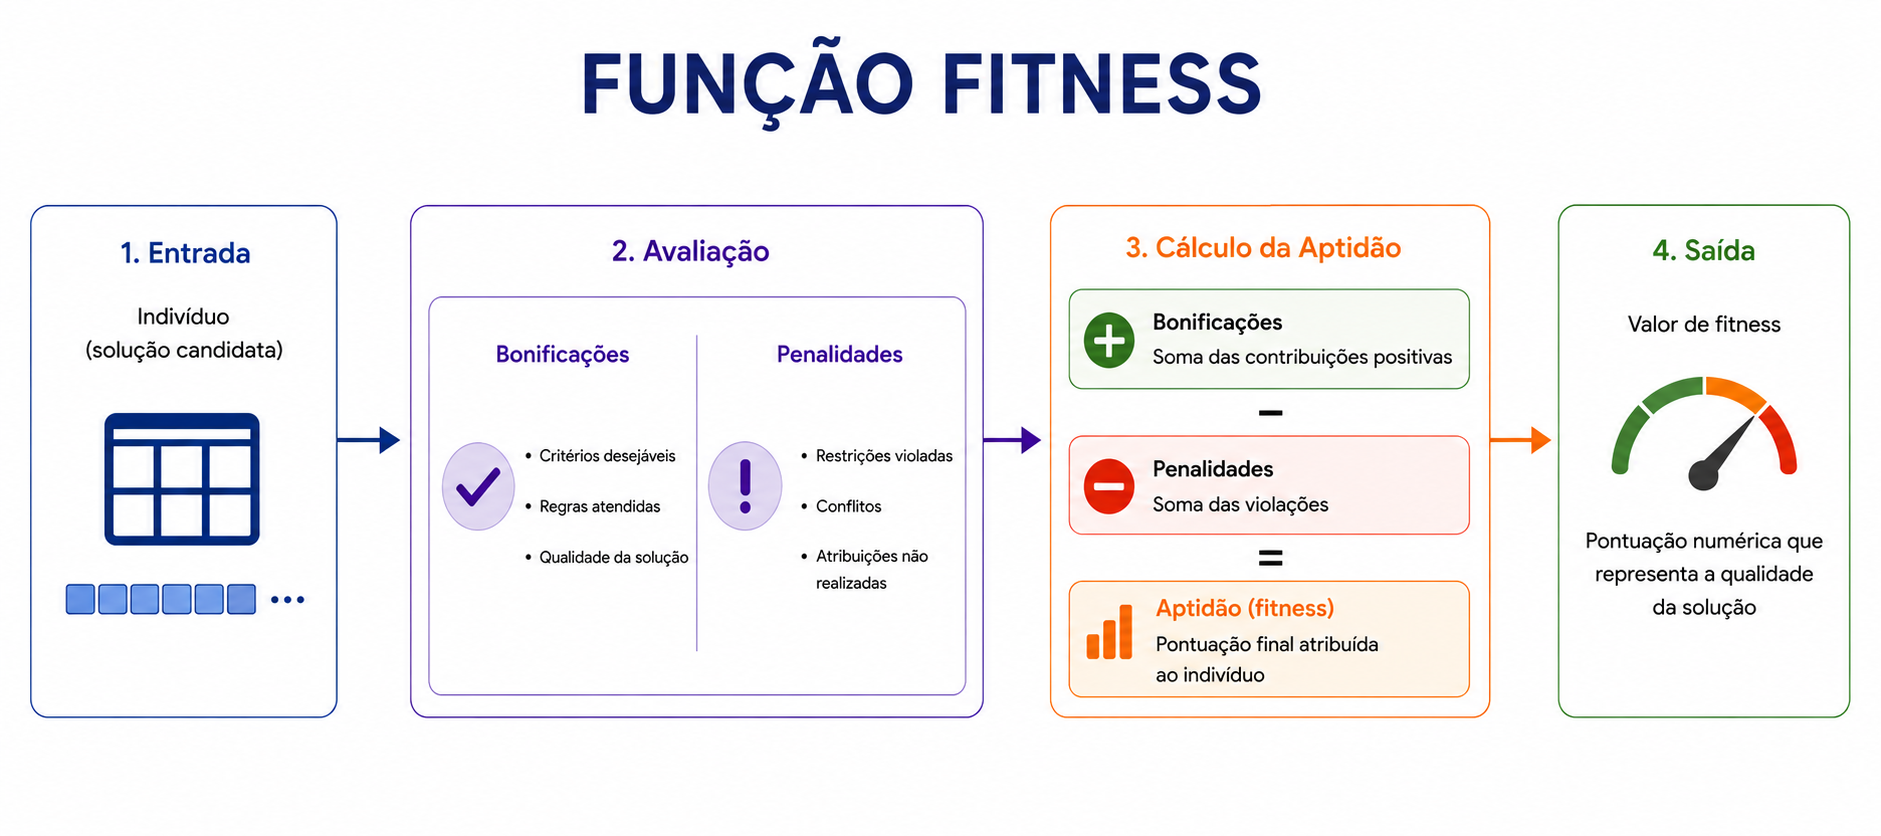
\includegraphics[width=0.85\textwidth]{figuras/Figura_1_ilustracaoFuncaoFitness.png}

\vspace{0.2cm}
\fonteautores
\end{figure}

\subsubsection{Seleção}
\label{subsubsec:selecao}

A seleção é o operador responsável por escolher quais indivíduos da população participarão do processo de reprodução e poderão contribuir para a formação da geração seguinte. Esse mecanismo representa, no contexto computacional, a pressão seletiva observada nos processos evolutivos naturais \cite{meniz2025}.

Em Algoritmos Genéticos, indivíduos com melhor valor de \textit{fitness} tendem a possuir maior probabilidade de serem selecionados. No entanto, a seleção não deve eliminar completamente indivíduos menos aptos, pois a manutenção de alguma diversidade populacional é importante para evitar a convergência prematura \cite{hussain2020}.

Entre os métodos de seleção mais utilizados estão a seleção por roleta, a seleção por torneio e a seleção por \textit{ranking}. A seleção por roleta atribui probabilidades proporcionais ao valor de \textit{fitness} de cada indivíduo. A seleção por torneio compara pequenos grupos de indivíduos e escolhe o mais apto entre eles. Já a seleção por \textit{ranking} considera a posição relativa dos indivíduos na população, reduzindo o impacto de diferenças absolutas muito grandes entre valores de aptidão \cite{meniz2025}.

\begin{figure}[H]
\centering
\caption{Seleção de indivíduos para reprodução em Algoritmos Genéticos}
\label{fig:selecao-individuos-ag}

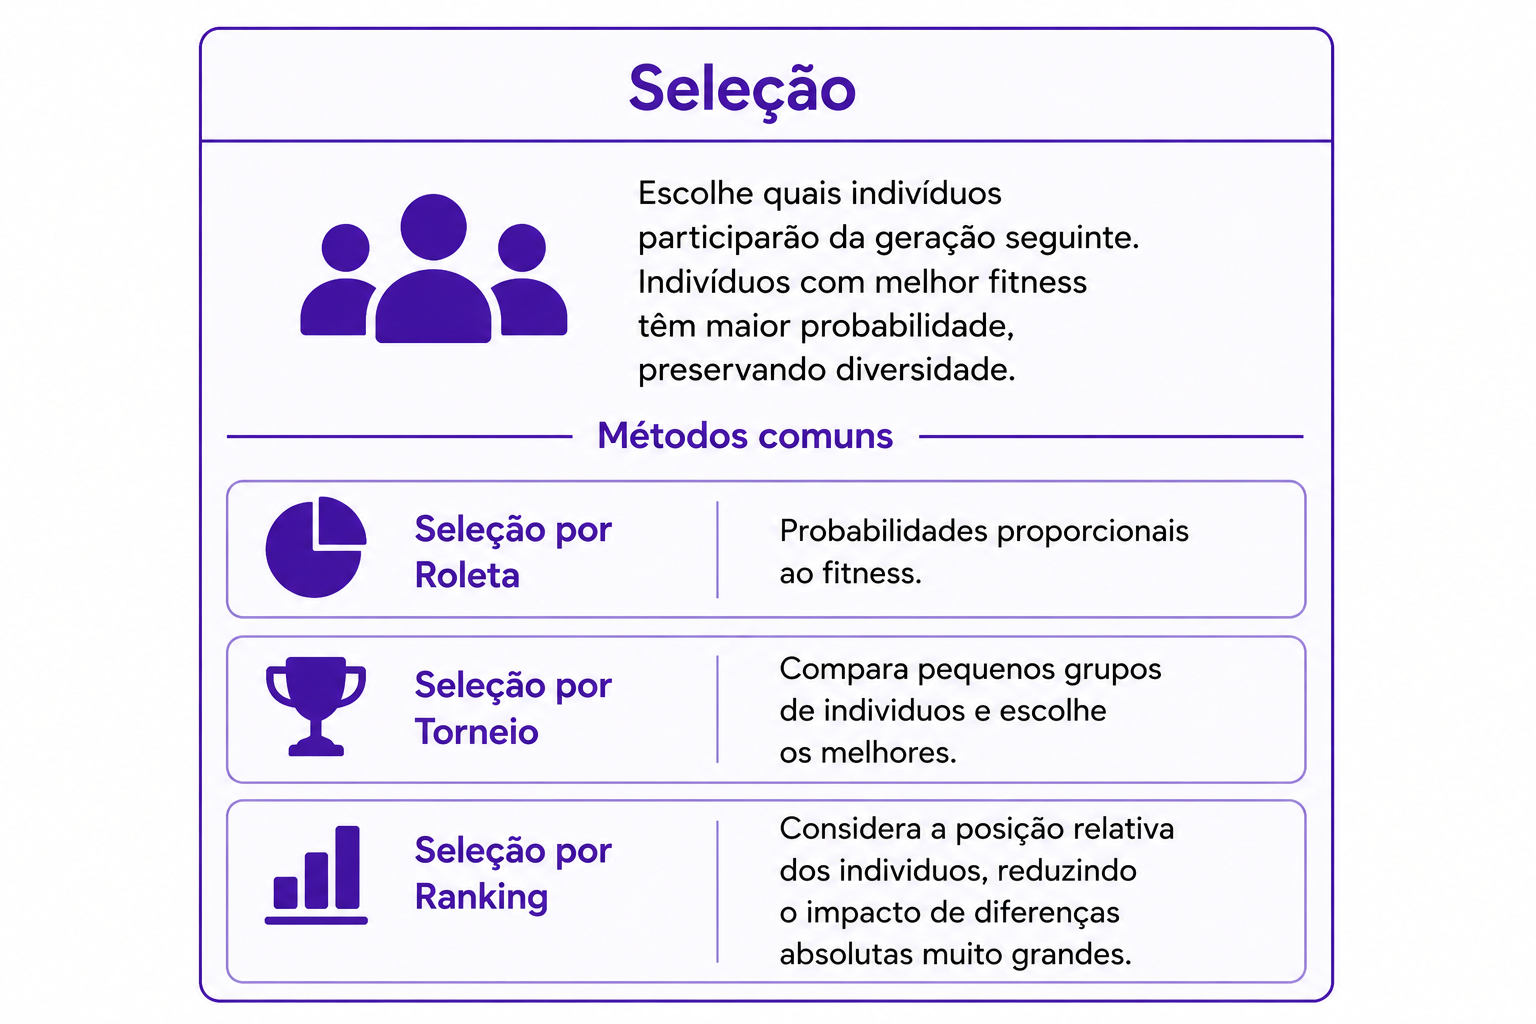
\includegraphics[width=0.85\textwidth]{figuras/Figura_2_ilustracaoAGSelecao.png}

\vspace{0.2cm}
\fonteautores
\end{figure}

\subsubsection{Crossover}
\label{subsubsec:crossover}

O \textit{crossover}, também chamado de cruzamento, corresponde ao operador de recombinação computacional. Sua função é combinar partes de dois ou mais indivíduos selecionados para gerar novos descendentes, preservando características de soluções consideradas promissoras \cite{umbarkar2015}.

Esse operador parte do princípio de que boas soluções podem conter componentes úteis que, quando recombinados com componentes de outras soluções, podem gerar indivíduos ainda mais adequados ao problema. Assim, o \textit{crossover} atua como mecanismo de exploração do espaço de busca, criando novas combinações a partir de informações já presentes na população \cite{fajrin2020}.

Existem diferentes estratégias de \textit{crossover}, como cruzamento de um ponto, cruzamento de múltiplos pontos e cruzamento uniforme. A escolha da estratégia depende da forma de codificação da solução e das restrições do problema. Em problemas de grades horárias, o operador deve ser projetado com cuidado, pois a troca inadequada de partes entre indivíduos pode gerar conflitos, como choques de professores, turmas ou horários \cite{umbarkar2015, fajrin2020}.

\begin{figure}[H]
\centering
\caption{Cruzamento de indivíduos em Algoritmos Genéticos}
\label{fig:crossover-ag}

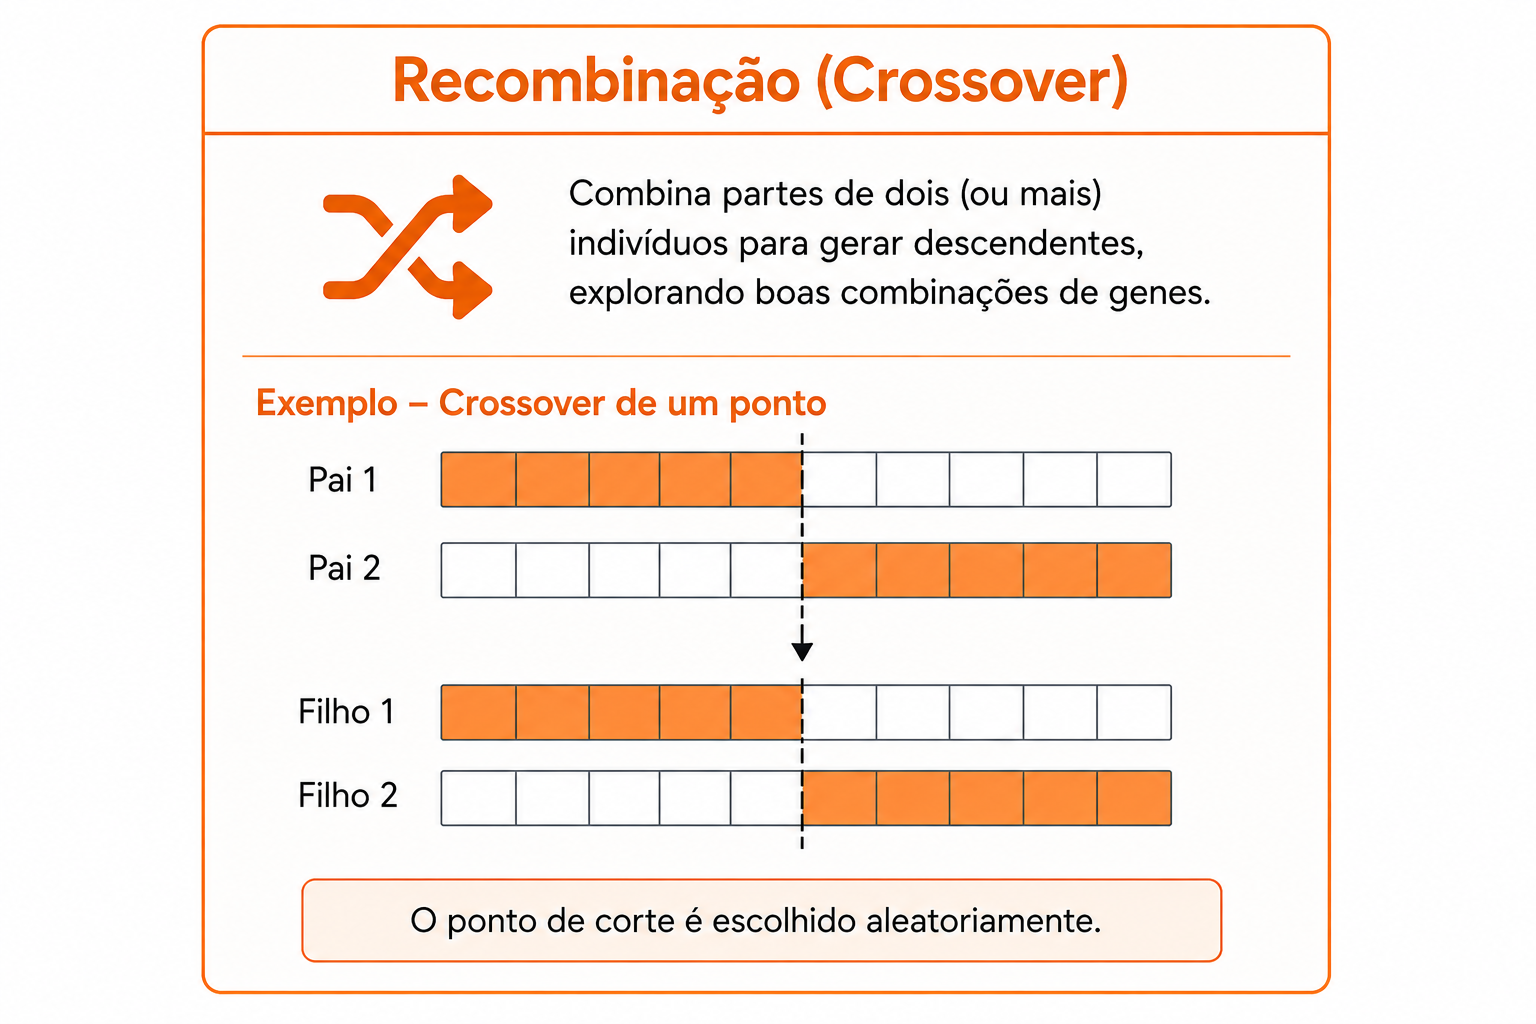
\includegraphics[width=0.85\textwidth]{figuras/Figura_3_ilustracaoAGCrossover.png}

\vspace{0.2cm}
\fonteautores
\end{figure}

\subsubsection{Mutação}
\label{subsubsec:mutacao}

A mutação é o operador responsável por introduzir alterações pontuais nos genes de um indivíduo. Seu papel é preservar a diversidade da população e permitir que o algoritmo explore regiões do espaço de busca que poderiam não ser alcançadas apenas por seleção e \textit{crossover} \cite{lengler2024}.

Em termos computacionais, a mutação pode modificar valores, trocar posições, substituir elementos ou alterar pequenas partes da solução, dependendo da representação adotada. Em um problema de timetabling universitário, por exemplo, uma mutação pode alterar o horário de uma aula, substituir uma alocação ou modificar a associação entre uma demanda acadêmica e determinado recurso disponível \cite{romaguera2024}.

Embora seja essencial para evitar a estagnação da busca, a mutação deve ser aplicada de forma controlada. Taxas muito baixas podem limitar a diversidade da população, enquanto taxas muito altas podem transformar o processo em uma busca excessivamente aleatória. Por isso, a taxa de mutação deve equilibrar exploração e estabilidade evolutiva \cite{cetin2020}.

Em problemas com muitas restrições, como o \textit{University Course Timetabling Problem} (UCTP), os operadores de seleção, \textit{crossover} e mutação exigem validação adicional, pois podem gerar soluções inválidas. Nesses casos, é comum empregar estratégias de penalização, reparo ou operadores especializados que preservem a viabilidade das soluções \cite{lagaros2023, romaguera2024}.

\begin{figure}[H]
\centering
\caption{Mutação em Algoritmos Genéticos}
\label{fig:mutacao-ag}

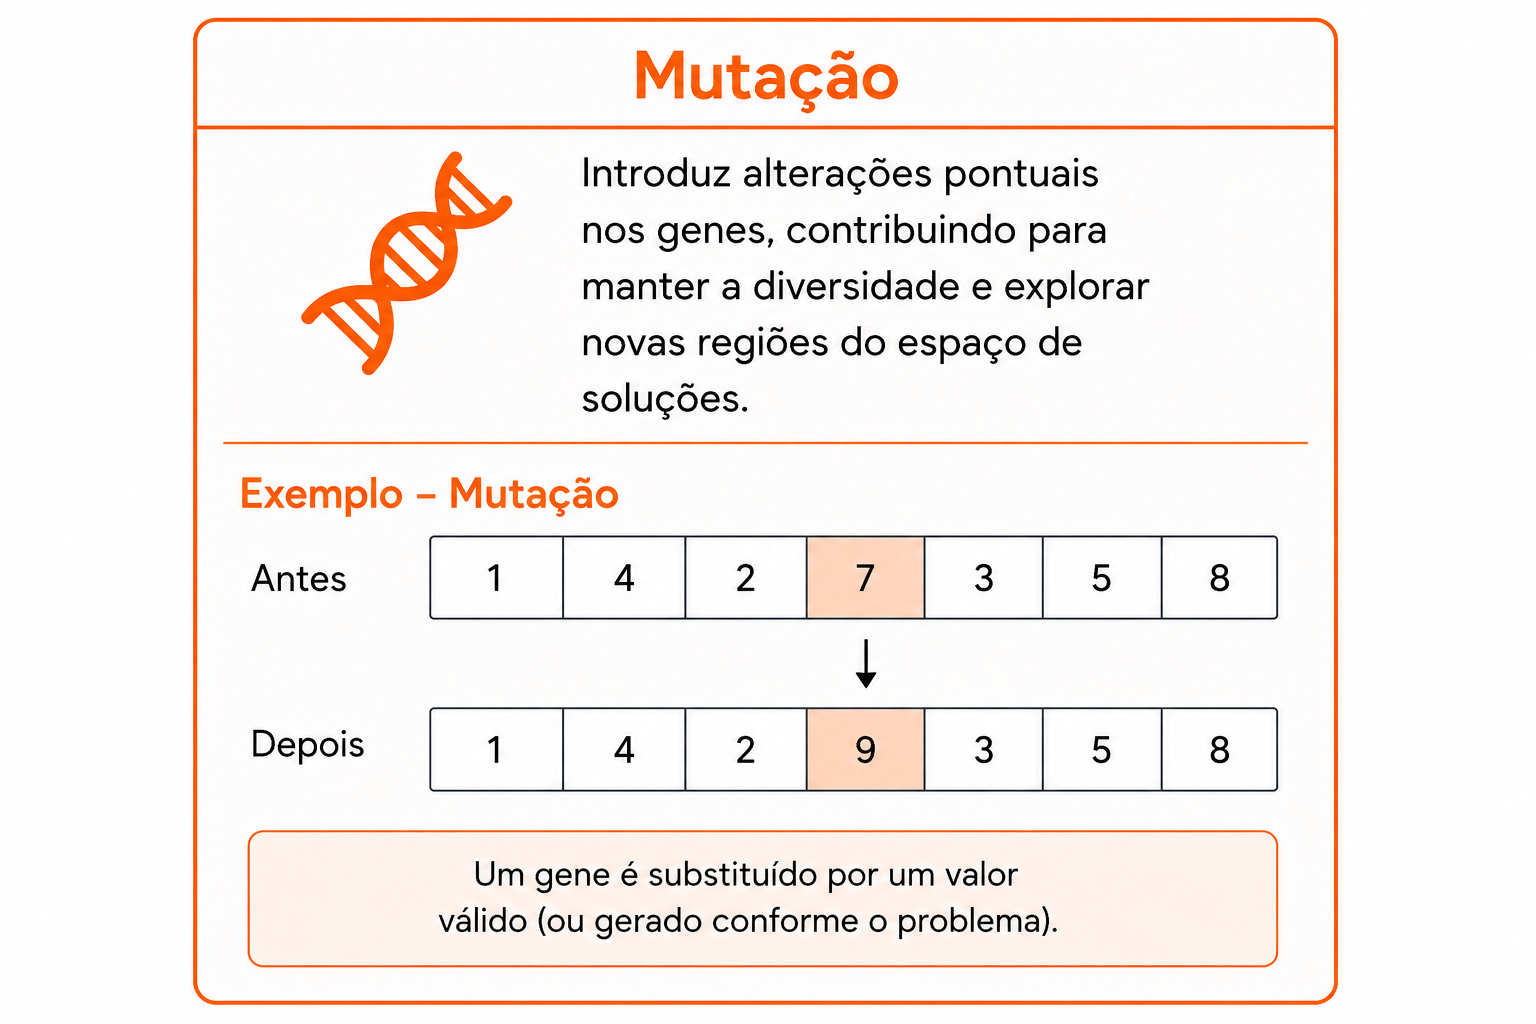
\includegraphics[width=0.85\textwidth]{figuras/Figura_4_ilustracaoAGMutacao.png}

\vspace{0.2cm}
\fonteautores
\end{figure}

\subsubsection{Tratamento de Restrições}
\label{subsubsec:tratamento-restricoes}

O tratamento de restrições é essencial em aplicações reais de Algoritmos Genéticos. Em problemas como o \textit{University Course Timetabling Problem} (UCTP), grande parte das combinações possíveis pode violar alguma regra, como conflito de professor, choque de turma ou incompatibilidade de horário \cite{abdipoor2023}.

As principais estratégias de tratamento incluem penalização, reparo, decodificação e operadores que preservam viabilidade. A penalização reduz o \textit{fitness} de soluções inválidas. O reparo tenta corrigir conflitos quando há alternativa possível. A decodificação transforma uma representação interna em uma solução válida. Já operadores restritivos buscam evitar a criação de indivíduos inviáveis desde o início \cite{rahimiConstraint2023, lagaros2023}.

A escolha da estratégia depende da natureza do problema e da forma como as restrições são modeladas. Em problemas altamente restritivos, a simples penalização pode não ser suficiente, pois a população pode permanecer concentrada em soluções inviáveis. Nesses casos, mecanismos de reparo ou operadores especializados tendem a contribuir para maior eficiência do processo evolutivo \cite{lagaros2023}.

\begin{figure}[H]
\centering
\caption{Tratamento de restrições em Algoritmos Genéticos}
\label{fig:tratamento-restricoes}

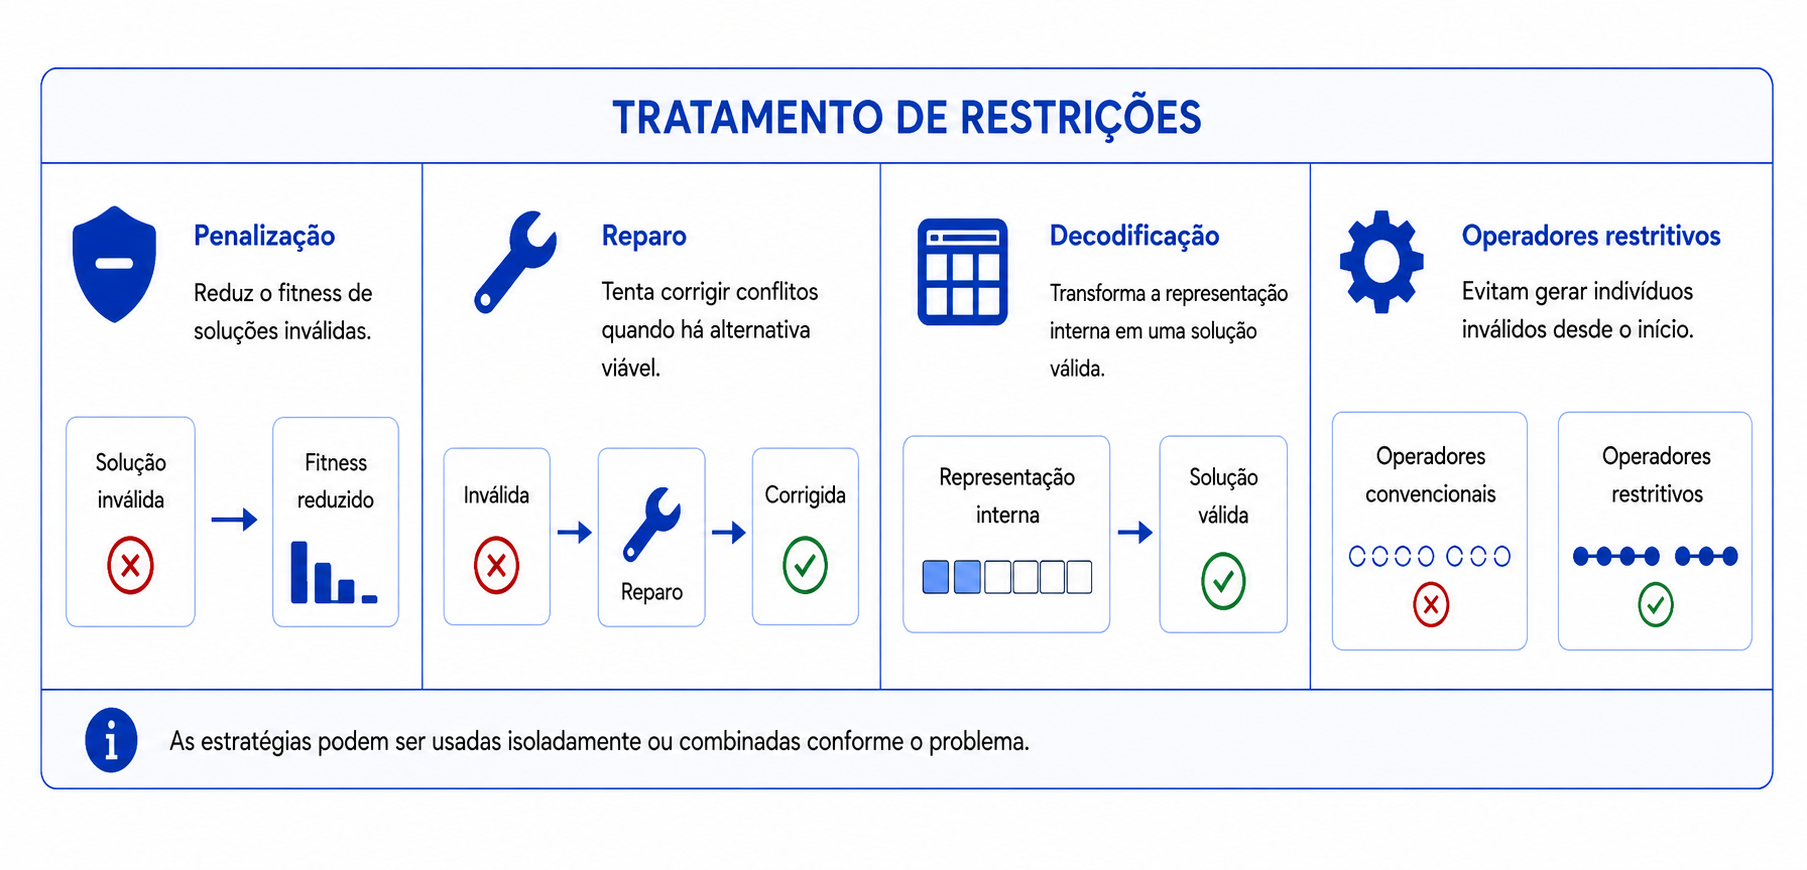
\includegraphics[width=0.85\textwidth]{figuras/Figura_5_ilustracaoAGTratamentoRestricoes.png}

\vspace{0.2cm}
\fonteautores
\end{figure}

\subsubsection{Convergência Prematura}
\label{subsubsec:convergencia-prematura}

Outro desafio importante em Algoritmos Genéticos é a convergência prematura. Esse fenômeno ocorre quando a população perde diversidade muito cedo e passa a se concentrar em uma região limitada do espaço de busca. Como consequência, o algoritmo pode estabilizar em uma solução localmente boa, mas distante de soluções potencialmente melhores \cite{cebeci2025}.

A convergência prematura está geralmente associada ao excesso de pressão seletiva, à baixa variabilidade introduzida pelos operadores genéticos ou ao uso inadequado de parâmetros. Fatores como tamanho da população, taxa de mutação, método de seleção e elitismo influenciam diretamente esse equilíbrio entre exploração e intensificação da busca \cite{cebeci2025, mustapha2026}.

Para reduzir esse problema, podem ser adotadas estratégias como aumento da diversidade populacional, ajuste da taxa de mutação, uso moderado de elitismo e escolha de métodos de seleção menos agressivos. Assim, busca-se preservar a capacidade de exploração do algoritmo ao longo das gerações, sem comprometer a evolução das soluções promissoras \cite{lengler2024, pytel2024}.

\begin{figure}[H]
\centering
\caption{Convergência Prematura em Algoritmos Genéticos}
\label{fig:convergencia-prematura}

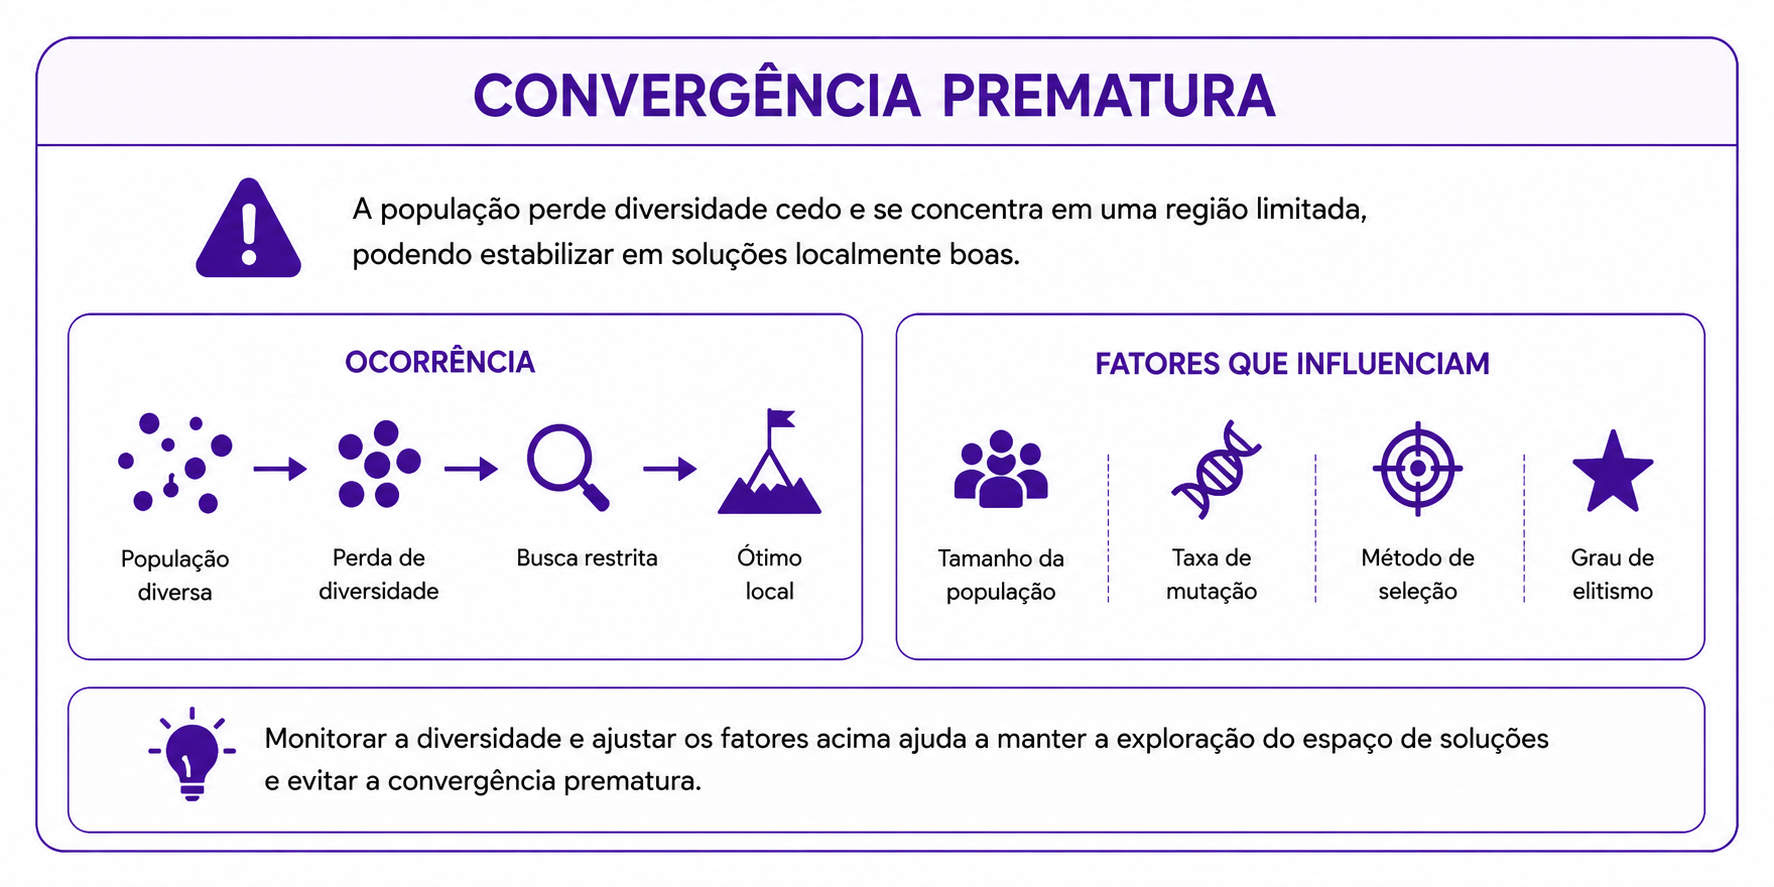
\includegraphics[width=0.85\textwidth]{figuras/Figura_6_ilustracaoAGConvergenciaPrematura.png}

\vspace{0.2cm}
\fonteautores
\end{figure}

\subsubsection{Ciclo de Execução e Pseudocódigo}
\label{subsubsec:ciclo-execucao-pseudocodigo}

O funcionamento geral de um Algoritmo Genético pode ser descrito como um ciclo evolutivo. Inicialmente, cria-se uma população de soluções candidatas. Em seguida, cada indivíduo é avaliado por uma função \textit{fitness}. Depois, o algoritmo seleciona indivíduos para reprodução, aplica \textit{crossover}, introduz mutações, avalia os novos indivíduos e forma uma nova população.

Esse processo é repetido até que o critério de parada seja satisfeito. Ao final, retorna-se a melhor solução encontrada segundo a função de avaliação adotada.

\begin{algorithm}[H]
\caption{Algoritmo Genético (BasicAG)}
\begin{enumerate}
\item População $\leftarrow$ InicializarPopulação()
\item AvaliarFitness(População)
\item repetir
\item Pais $\leftarrow$ SelecionarPais(População)
\item Filhos $\leftarrow$ Cruzamento(Pais)
\item Filhos $\leftarrow$ Mutação(Filhos)
\item AvaliarFitness(Filhos)
\item População $\leftarrow$ Substituir(População, Filhos)
\item até CritérioDeParadaSatisfeito()
\item retornar MelhorSolução(População)
\end{enumerate}
\end{algorithm}


\begin{figure}[H]
\centering
\caption{Representação gráfica do ciclo de execução de um Algoritmo Genético}
\label{fig:ilustracao-ag}

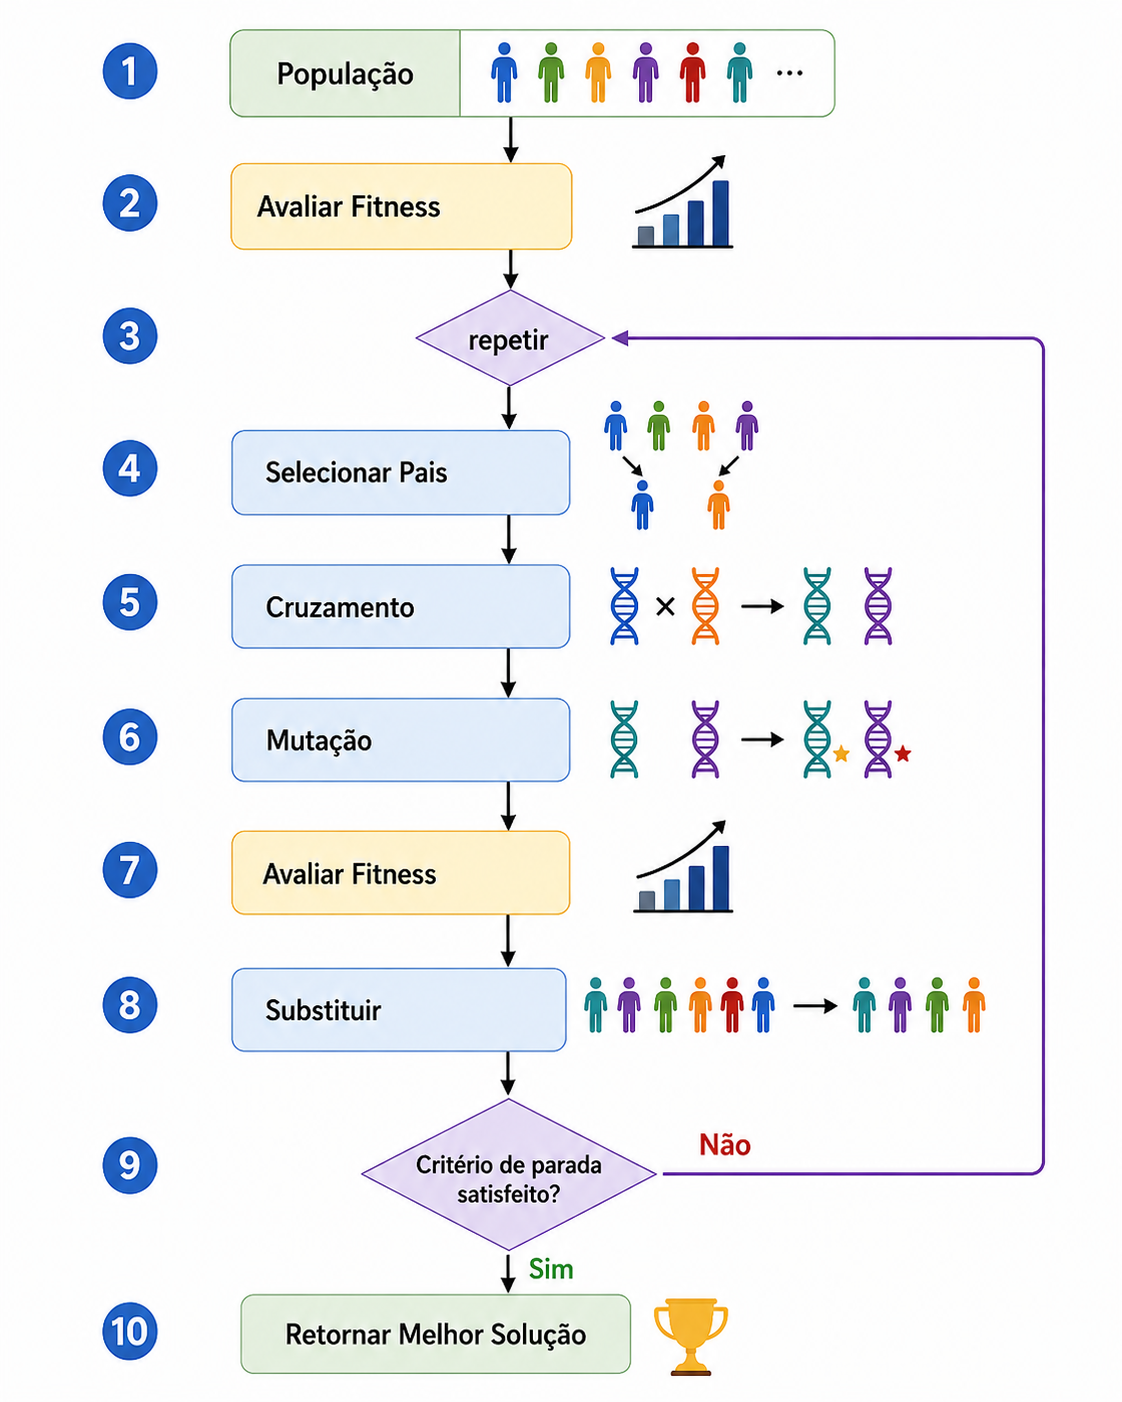
\includegraphics[width=0.85\textwidth]{figuras/Figura_7_ilustracaoAG.png}

\vspace{0.2cm}
\fonteautores
\end{figure}


Esse fluxo representa a estrutura geral dos Algoritmos Genéticos. Sua eficácia depende da adequação entre representação, função \textit{fitness}, operadores genéticos, tratamento de restrições e critérios de parada. No contexto do IGRIS, essa lógica fundamenta a geração automatizada de grades horárias acadêmicas, posteriormente detalhada nos capítulos de implementação.
